\documentclass{article}%
\usepackage[T1]{fontenc}%
\usepackage[utf8]{inputenc}%
\usepackage{lmodern}%
\usepackage{textcomp}%
\usepackage{lastpage}%
\usepackage[head=40pt,margin=0.5in,bottom=0.6in]{geometry}%
\usepackage{graphicx}%
%
\title{\textbf{Ministerio de Salud: 16 toneladas de medicamentos llegan al país para más de 400 mil pacientes}}%
\author{AVN}%
\date{19/09/2018}%
%
\begin{document}%
\normalsize%
\maketitle%
\textbf{URL: }%
http://www.eluniversal.com/economia/21064/ministerio{-}de{-}salud{-}16{-}toneladas{-}de{-}medicamentos{-}llegan{-}al{-}pais{-}para{-}mas{-}de{-}400{-}mil{-}pacientes\newline%
%
\textbf{Periodico: }%
EU, %
ID: %
21064, %
Seccion: %
economia\newline%
%
\textbf{Palabras Claves: }%
NO\_TIENE\newline%
%
\textbf{Derecho: }%
2.1%
, Otros Derechos: %
NO\_TIENE%
, Sub Derechos: %
2.1.2%
\newline%
%
\textbf{EP: }%
NO\newline%
\newline%
%
\textbf{\textit{El cargamento de medicamentos será distribuido por un lapso de tres meses, sobre todo en 18 hospitales ubicados en Sucre, Lara, Zulia, Delta Amacuro, Amazonas, Bolívar, Monagas, entre otros}}%
\newline%
\newline%
%
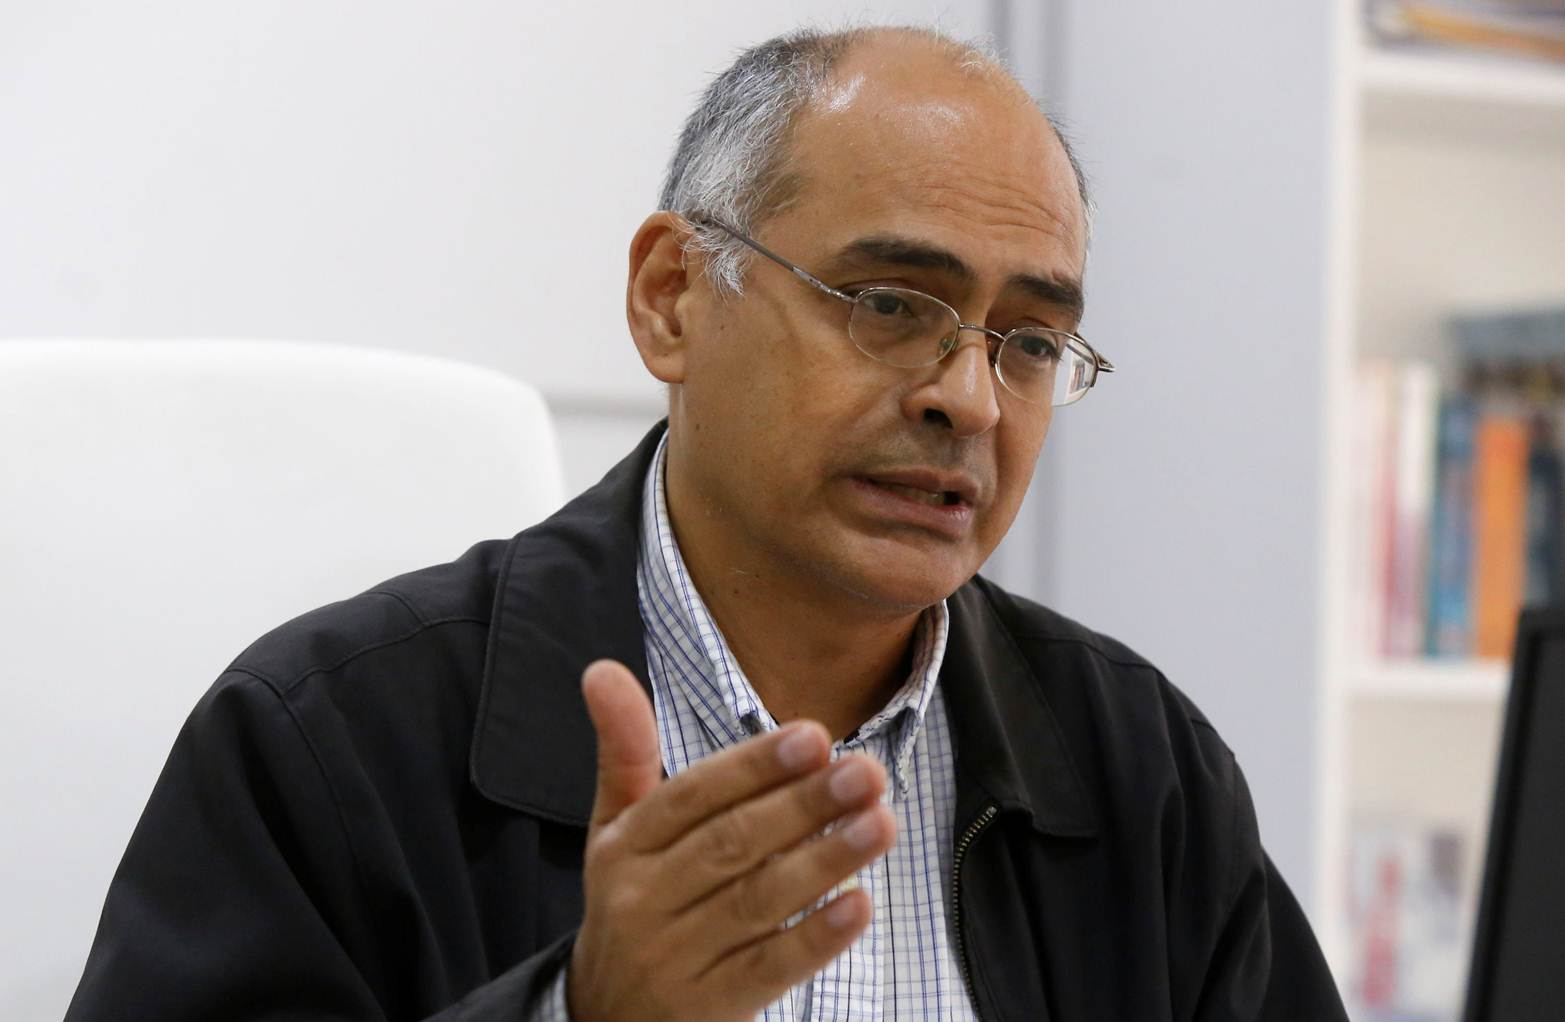
\includegraphics[width=300px]{51.jpg}%
\newline%
%
Caracas.{-} Un total de 16 toneladas de medicamentos serán distribuidas en el territorio nacional para más de 400 mil pacientes por un lapso de tres meses, informó el Ministerio para la Salud.%
\newline%
%
Este lote de medicinas llegó esta semana al país, en el marco de la cooperación entre el Gobierno nacional con la Organización Panamericana de la Salud (OPS) y la Organización Mundial de la Salud (OMS), reseñó AVN.%
\newline%
%
En nota de prensa se precisa que 40 kits serán enviados a 18 hospitales que han sido priorizados y que están ubicados en los estados Sucre, Lara, Zulia, Delta Amacuro, Amazonas, Bolívar, Monagas, entre otros.%
\newline%
%
En esta ocasión, se incrementa el número de instalaciones asistenciales que reciben esta dotación, tomando en cuenta que en la entrega anterior fueron 11 instituciones de salud a las que se les hizo entrega, según información del Gobierno.%
\newline%
%
El ministerio subrayó que en el transcurso de tres meses, el inventario se va a reponer para "garantizar la protección" de la población venezolana.%
\newline%
%
Asimismo, destacó que pese al supuesto "bloqueo económico" al que ha sido "sometido" Venezuela por parte del gobierno de Estados Unidos y sus aliados internacionales, el Ejecutivo realiza "esfuerzos" para la adquisición de medicamentos y material médico%
\newline%
%
\end{document}